%\lipsum[4-4]
In this chapter is presented the development of the wireless monitoring system, following the specifications and requirements raised in the chapter 2. This chapter is divided in four parts, starting with the description of the selected wireless technology. In \ref{sec:3.2} and \ref{sec:3.3} is presented the hardware and software architecture of the system. Communication results and KPI metrics are presented in section \ref{sec:3.4}. In section \ref{sec:3.5} is made the discussion of the results.

\section{Description of the selected wireless technology}
\label{sec:3.1}
%\lipsum[4-4]

The CC1350 platform was selected to fulfill the wireless requirements. The availability of Sub-1 GHz and Bluetooth technologies in the same device allows enough flexibility in terms of possible functionalities to be implemented. The powerful 32-bit ARM Cortex-M3 allows the implementation of a Real-time Operating System, capable of handling several tasks.

\section{Hardware architecture}
\label{sec:3.2}
%\lipsum[4-4]

The hardware architecture depends on serial communication between the power converter and the wireless node. Complementary, it depends on serial communication between the concentrator and the end user applications (serial monitor, Raspberry Pi and concentrator LCD). Figure \ref{fig:3.2.hw} presents the hardware architecture.

\begin{figure}[h!]
	\centering
	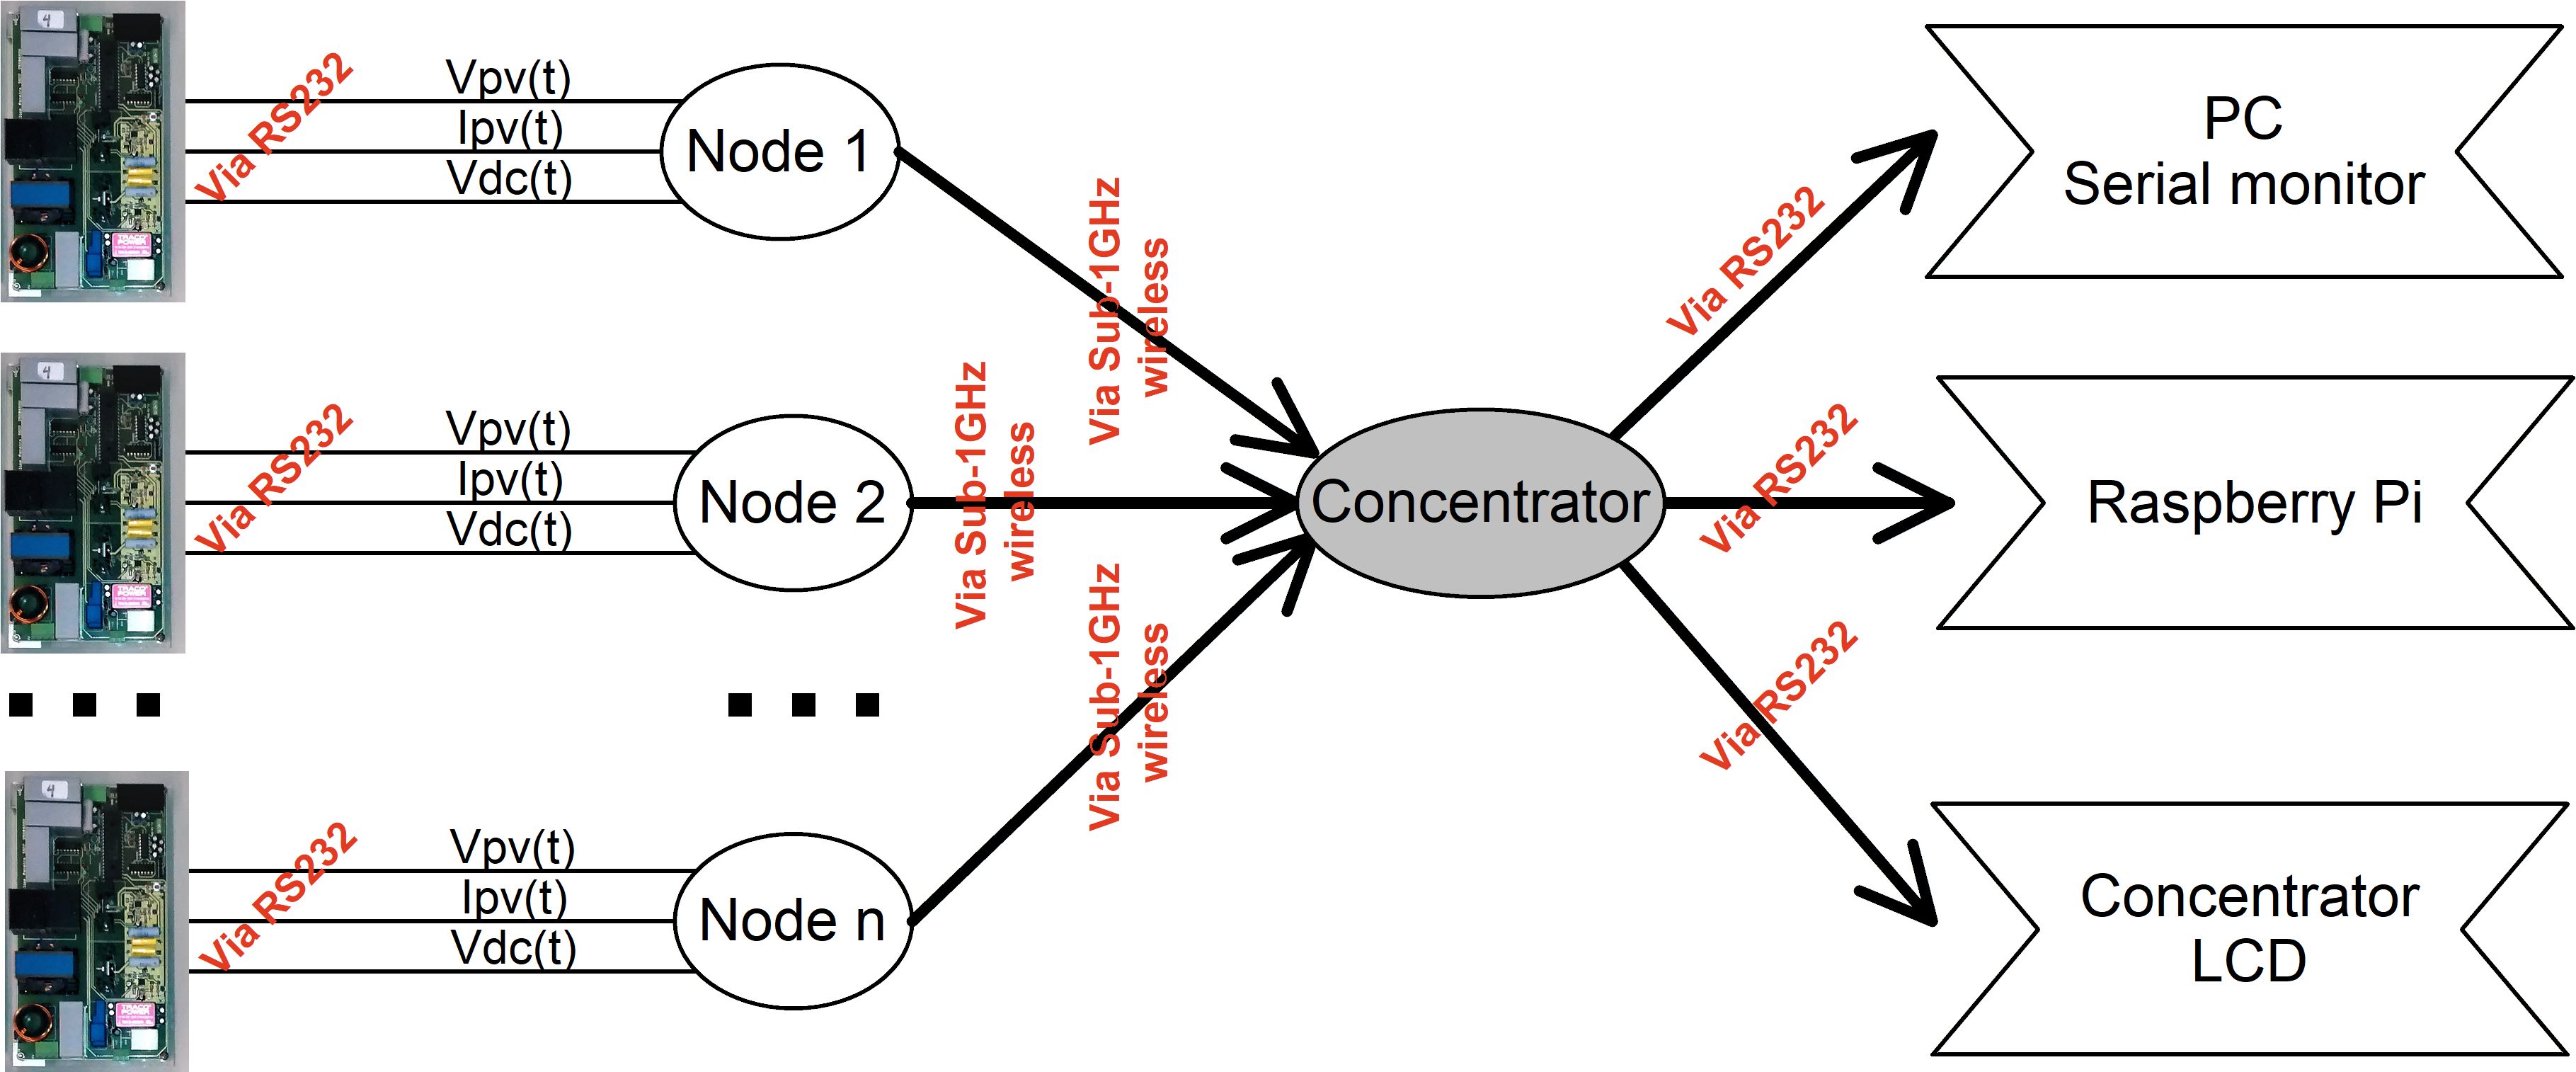
\includegraphics[width=0.9\textwidth,keepaspectratio]{figures/hw}
	\caption{Hardware architecture.}
	\label{fig:3.2.hw}
\end{figure}

The communication interface between node and power converter must support different voltage levels (in particular 3.3V from CC1350 node and 5V from power converter). This way, an electronic board (PCB) was developed to support this constraint. Complementary, this PCB allows a robust mechanical interface between the wireless node and the power converter, without extending the dimensions defined in the SRS. This PCB integration with wireless node and the power converter is presented in the figure \ref{fig:3.2.pcb}.

\begin{figure}[h!]
	\centering
	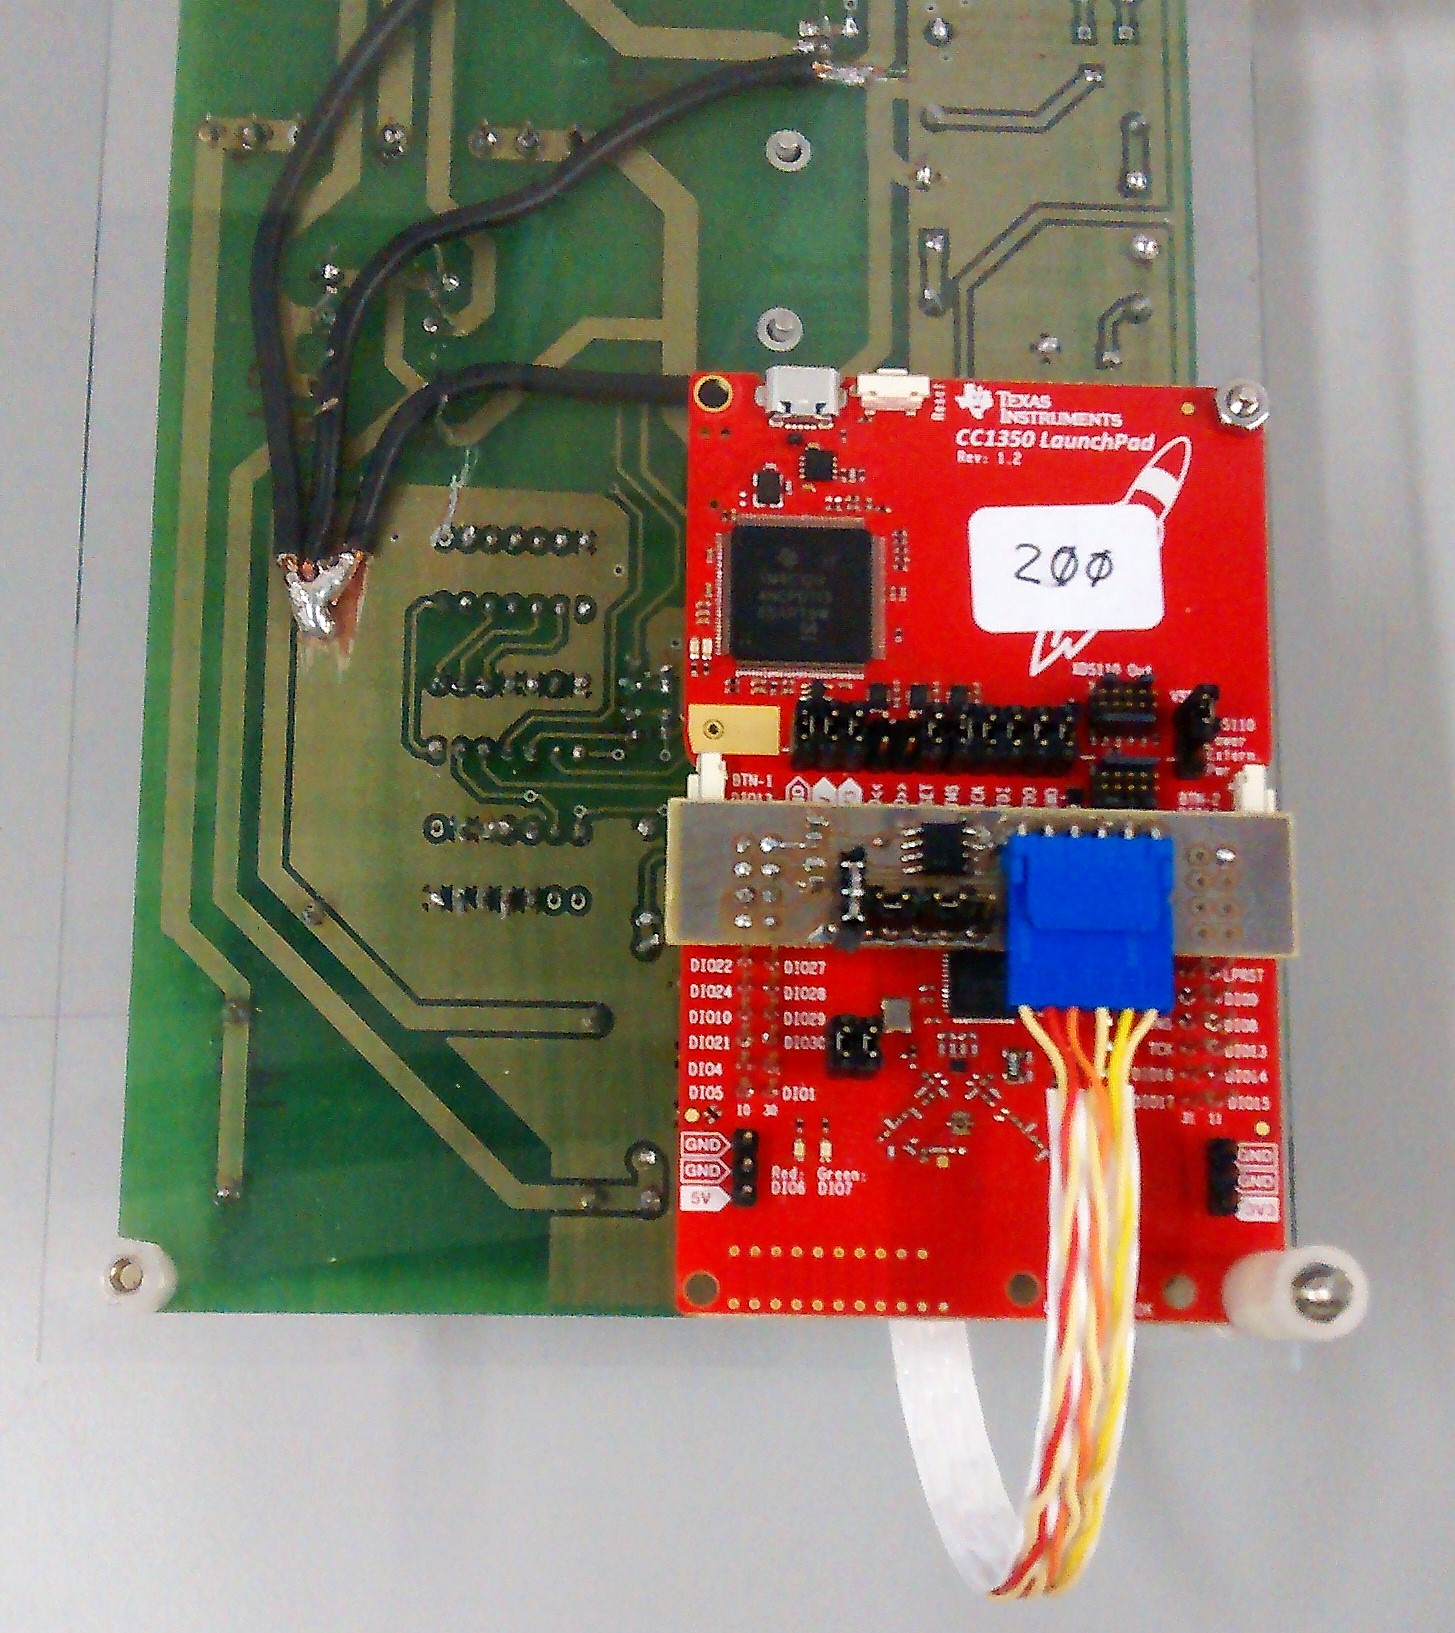
\includegraphics[width=0.4\textwidth,keepaspectratio]{figures/pcb}
	\caption{PCB integration with wireless node and the power converter.}
	\label{fig:3.2.pcb}
\end{figure}

On the concentrator side, the CC1350 development board has available the USB serial communication as well as the LCD as shown in figure \ref{fig:3.2.concentr}.

\begin{figure}[h!]
	\centering
	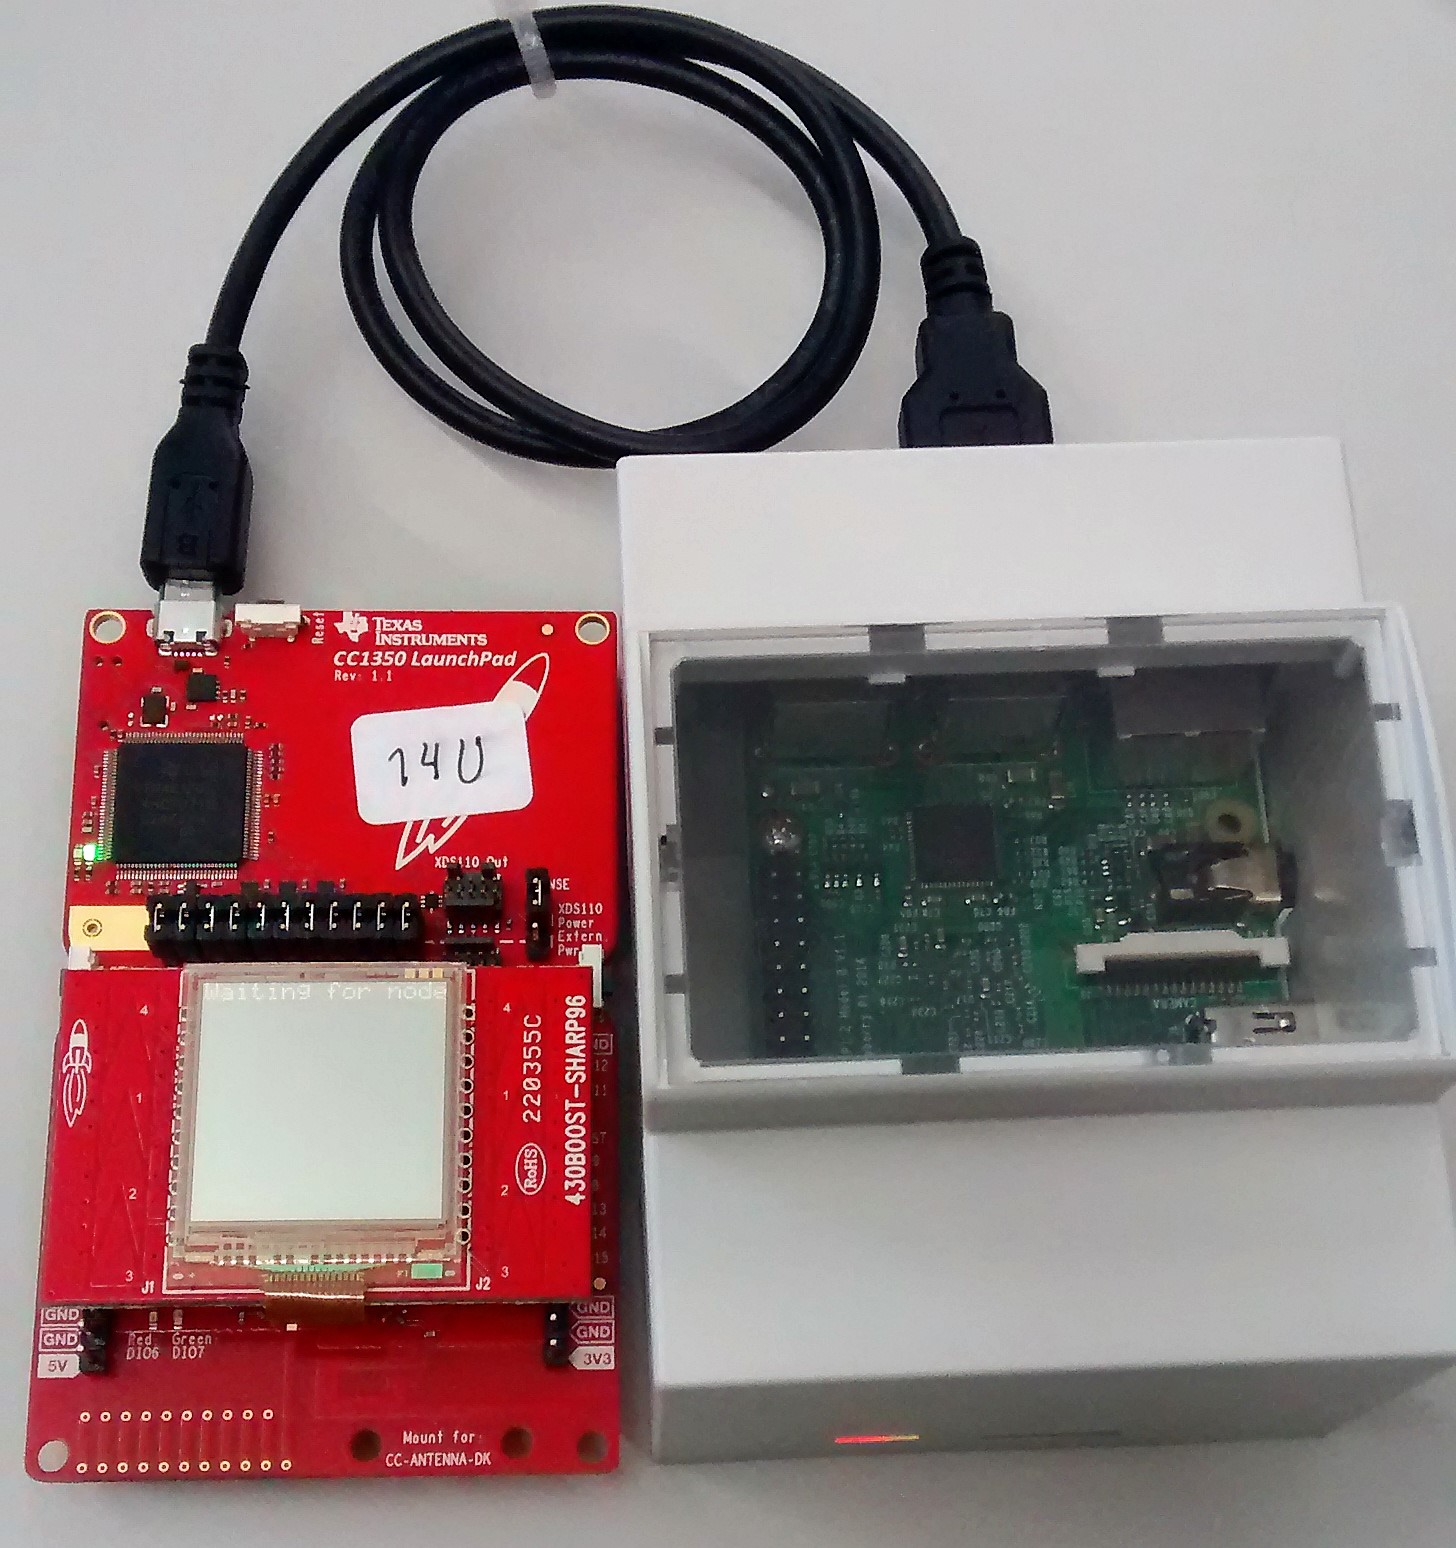
\includegraphics[width=0.5\textwidth,keepaspectratio]{figures/concentr}
	\caption{Concentrator connected to RPI.}
	\label{fig:3.2.concentr}
\end{figure}

\section{Software Architecture}
\label{sec:3.3}
%\lipsum[4-4]

As proposed in the SRS, figure \ref{fig:3.3.domainModel} presents the domain model of the software to be implemented in the concentrator and nodes.

\begin{figure}[h!]
	\centering
	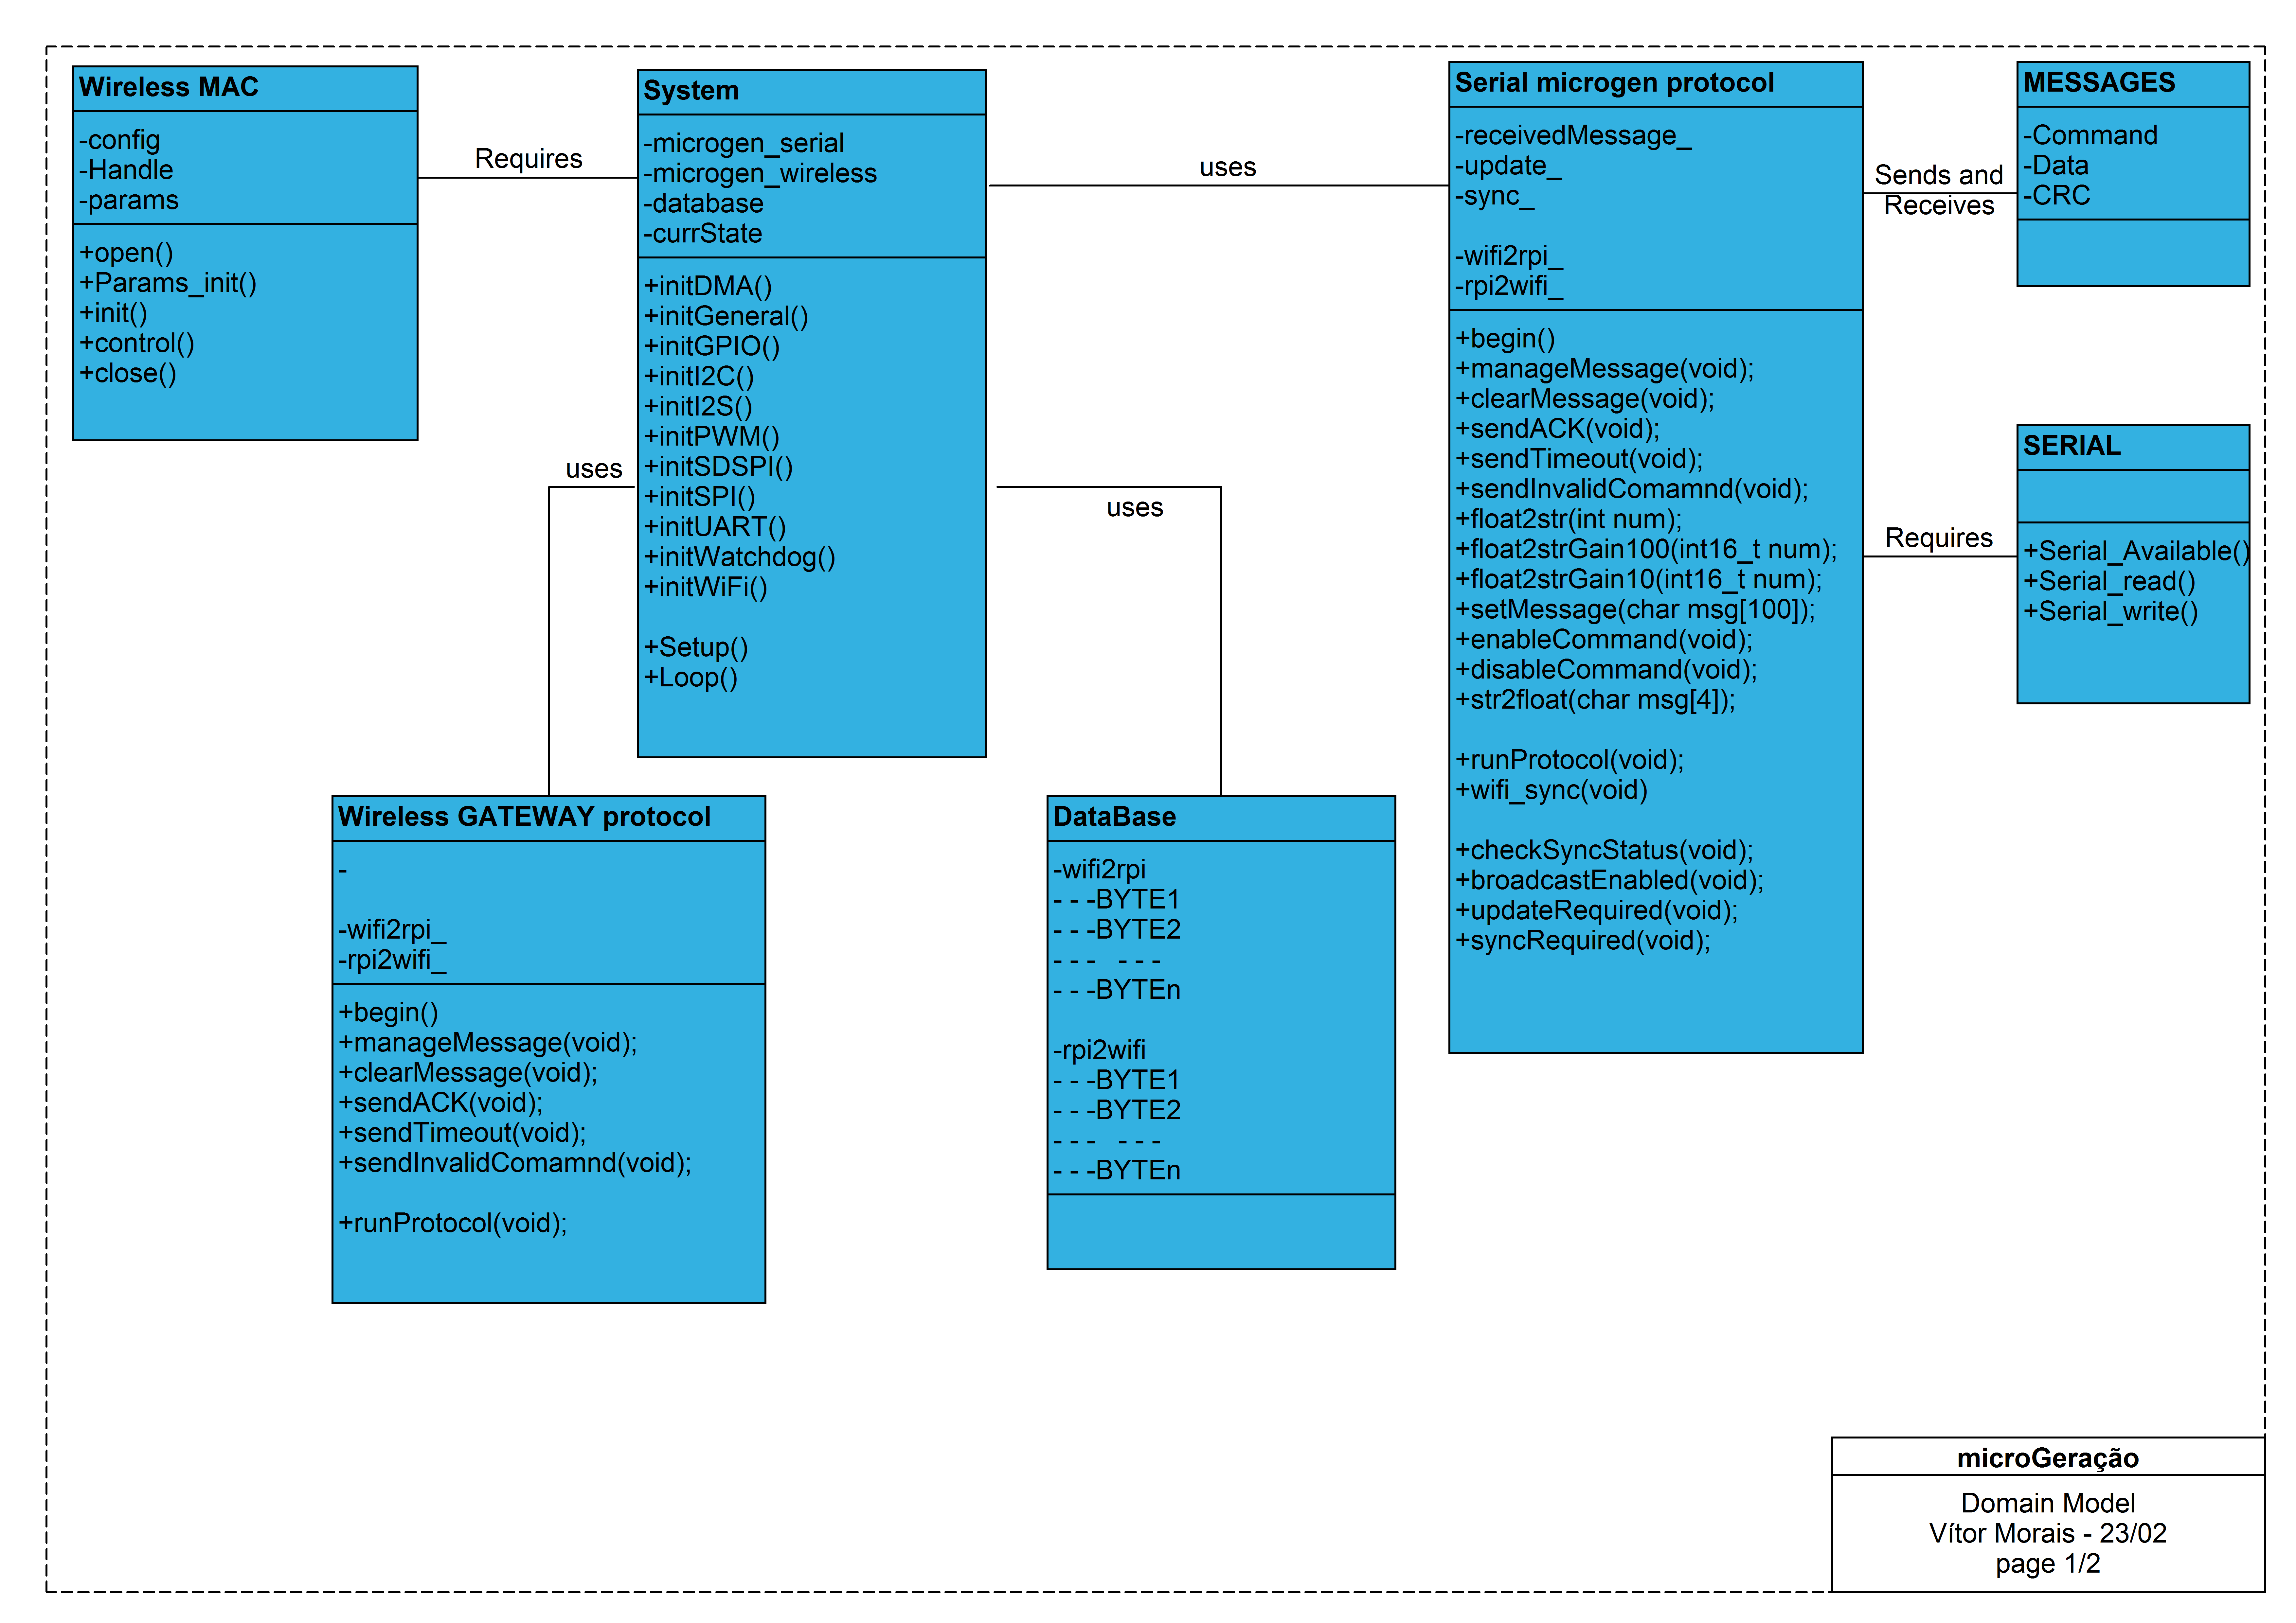
\includegraphics[width=0.85\textwidth,keepaspectratio]{figures/domainModel}
	\caption{Domain Model Diagram.}
	\label{fig:3.3.domainModel}
\end{figure}

The software architecture was based on a proprietary implementation of a WSN by the manufacturer of the CC1350 (Texas Instruments). In the power converter side, a serial request-response protocol was implemented. In addition, the database was constructed based on flowchart of figure \ref{fig:3.3.sw1}. 

\begin{figure}[h!]
	\centering
	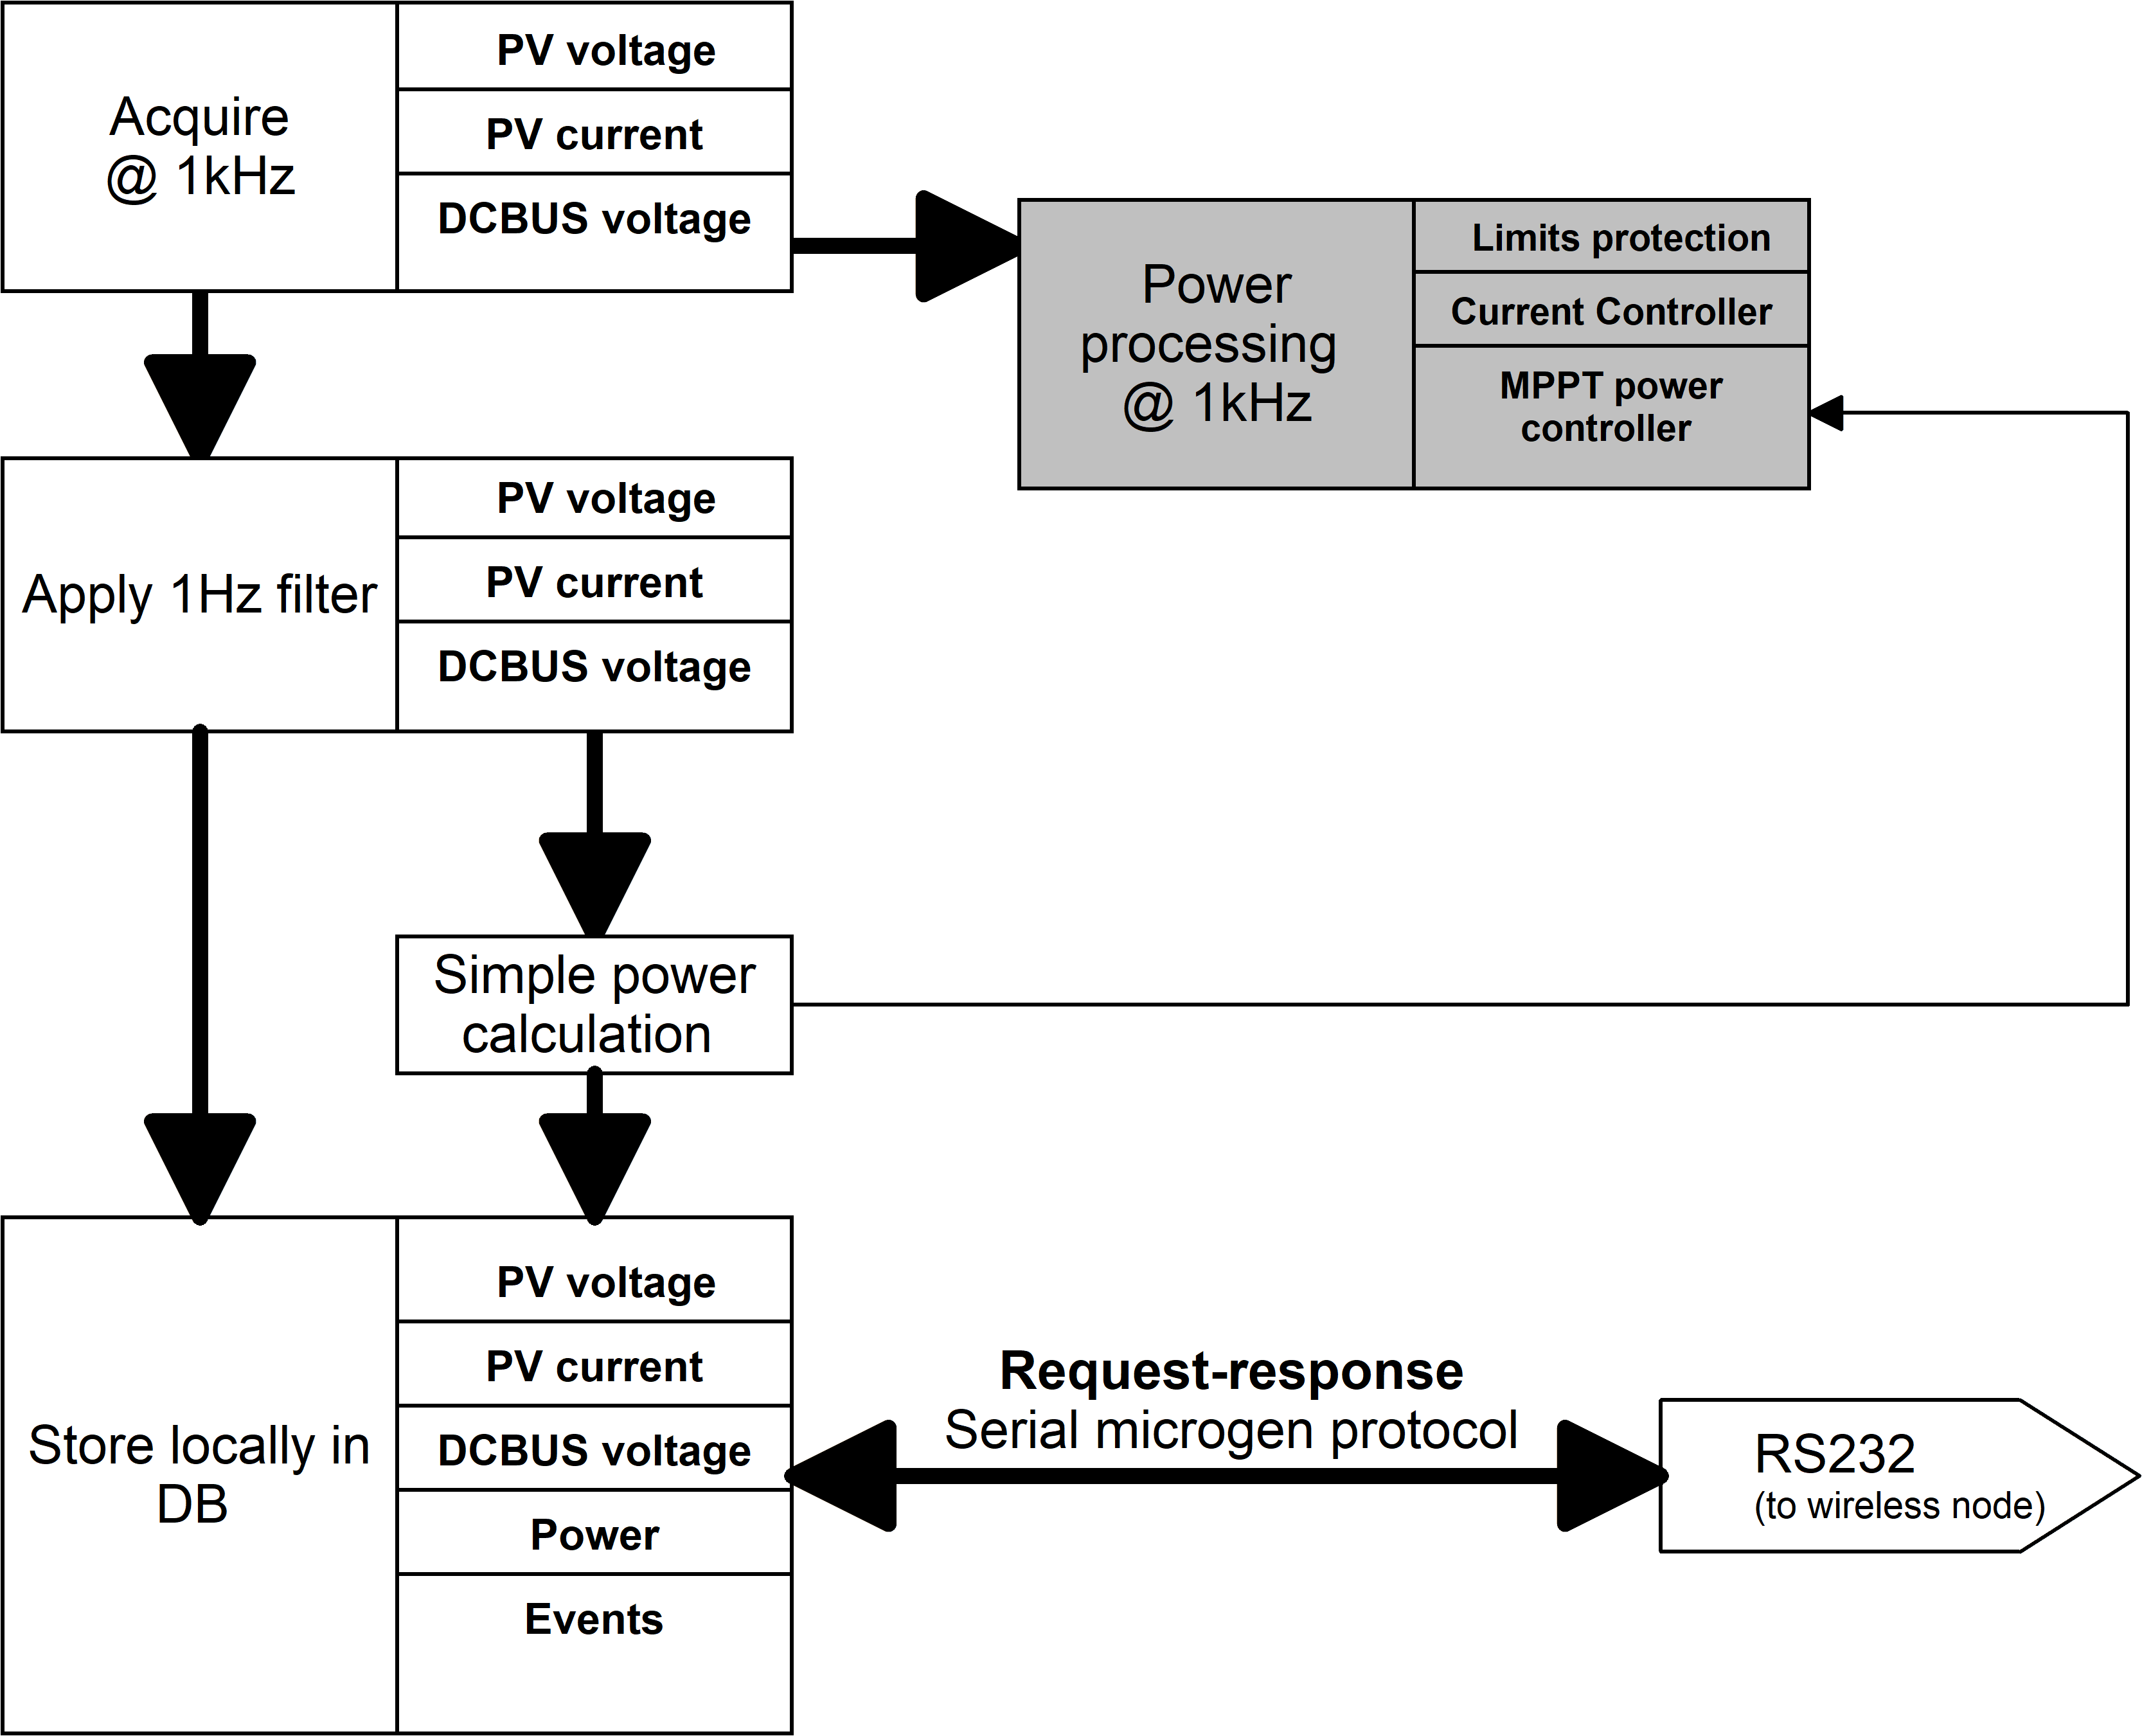
\includegraphics[width=0.55\textwidth,keepaspectratio]{figures/sw1}
	\caption{PV power converter implemented software.}
	\label{fig:3.3.sw1}
\end{figure}


The power converter acts as a communication slave that responds upon wireless node requests. The following list presents the data exchange between both devices:
\begin{description}
	\setlength\itemsep{-0.5em}
	\item[\#VPV\#03\#] Request for panel voltage, with 0,1V precision;
	\item[\#IPV\#03\#] Request for panel current, with 0,01A precision;
	\item[\#VDC\#03\#] Request for DC Bus voltage, with 1V precision;
	\item[\#PWR\#03\#] Request for PV power, with 1W precision;
	\item[\#EVE\#03\#] Request for PV power converter events;
	\item[\#WHOIS\#05\#] Request for board identification.
	\item[\#SYNC\#04\#] Request for Database synchronization.
\end{description}

The remote node will request for the values in the PV power converter database. At a 1 second period, the data is sent to the data concentrator.

\section{Communication results}
\label{sec:3.4}
%\lipsum[4-4]
In figure \ref{fig:3.4.armario1} and \ref{fig:3.4.armario2} is presented the pretended test-bench for the wireless nodes. 
\begin{figure}[!htb]
	\centering
	\begin{minipage}{.55\textwidth}
		\centering
		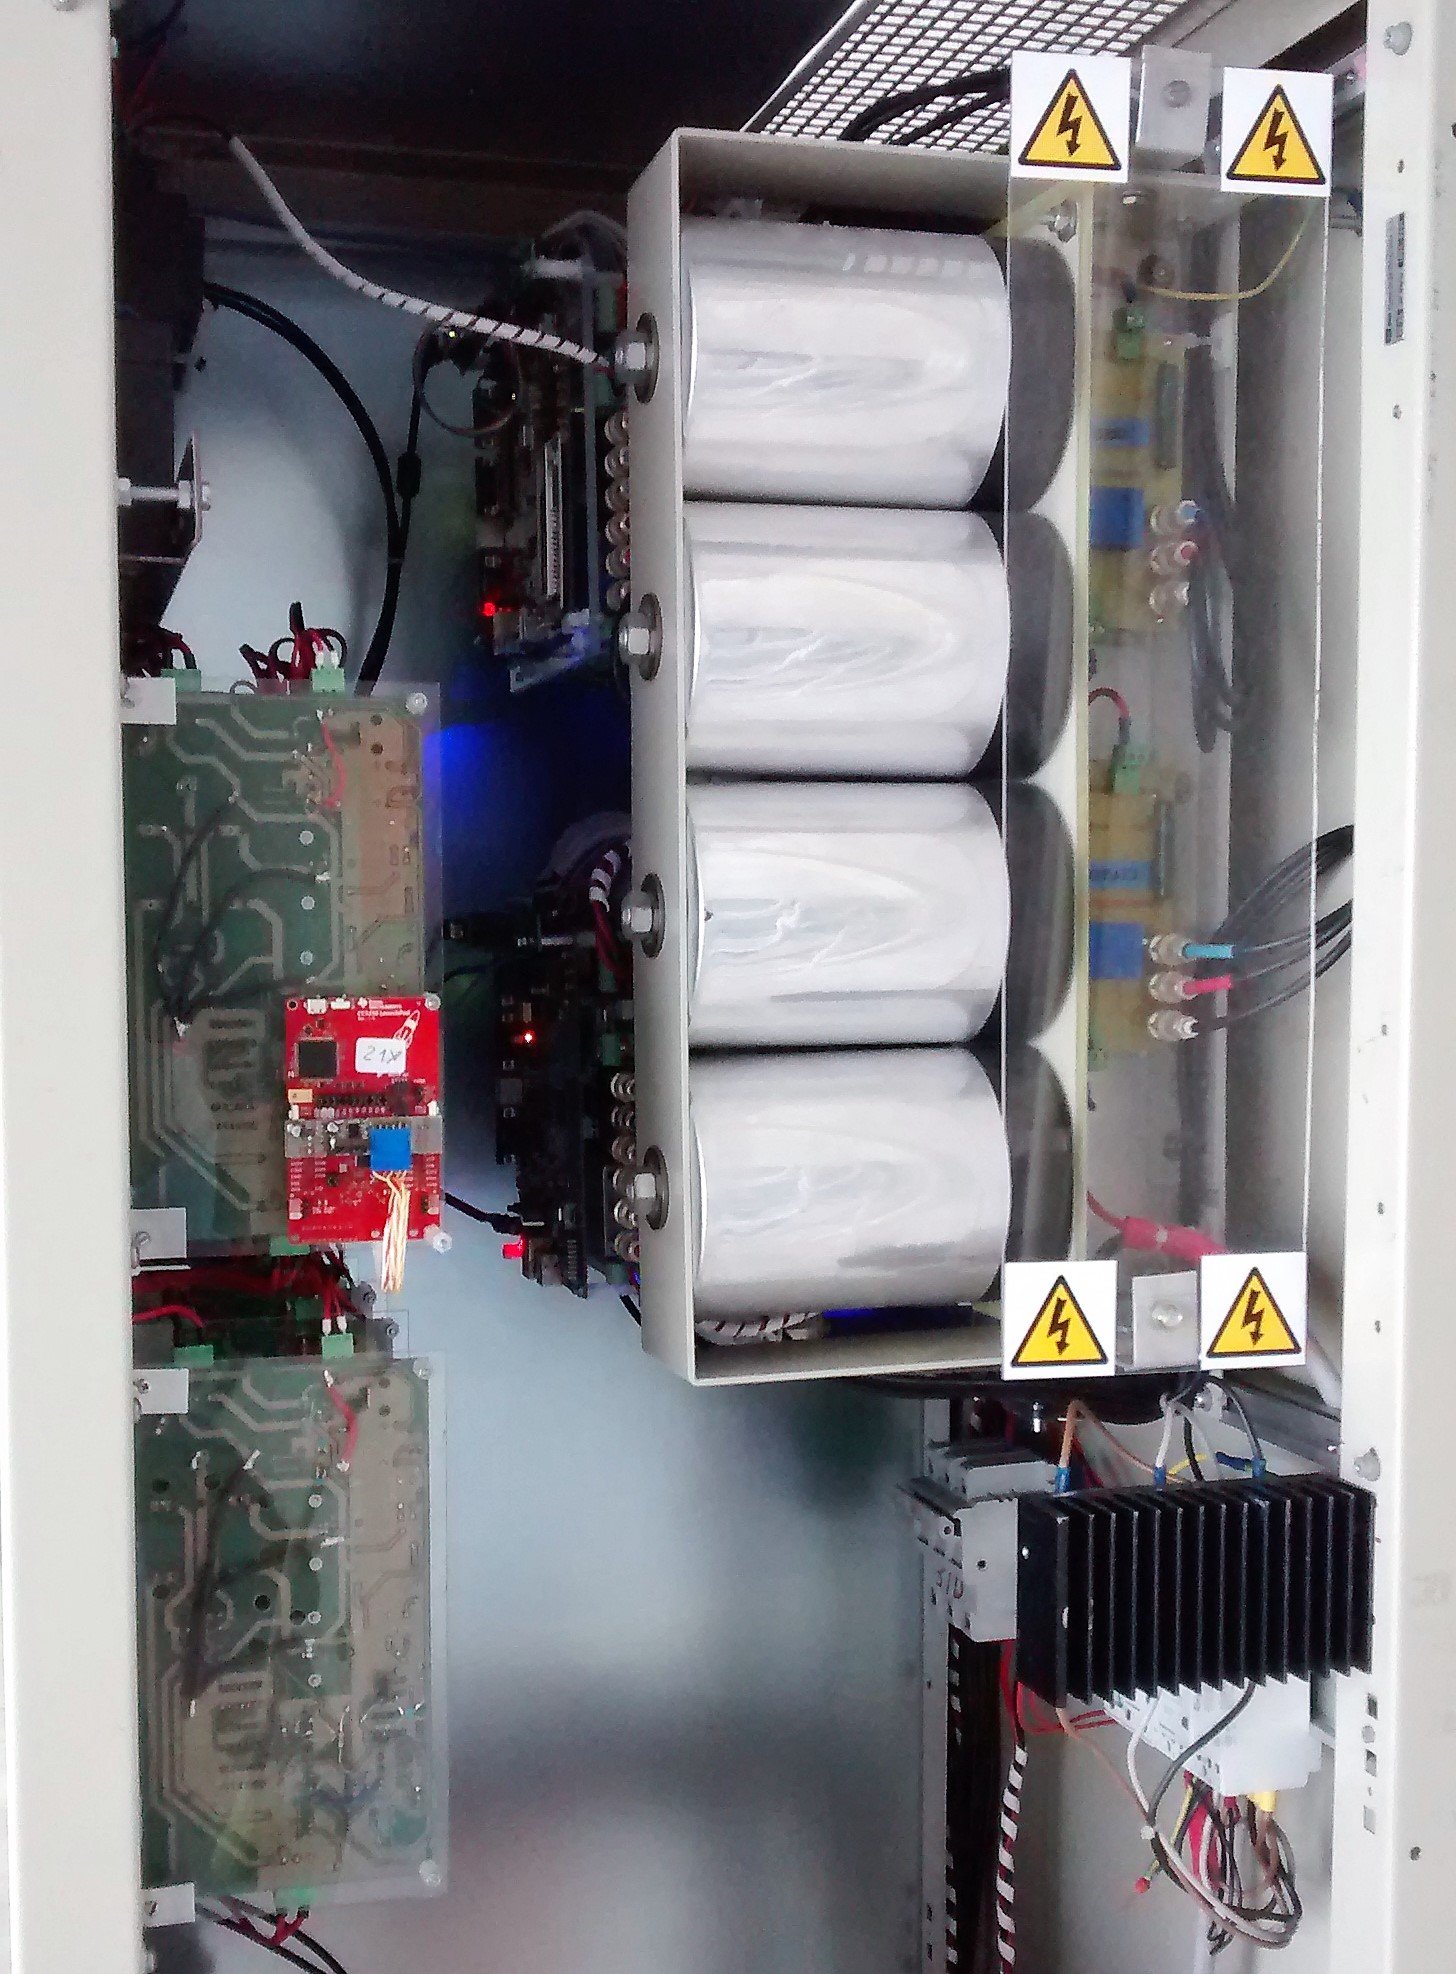
\includegraphics[width=0.75\linewidth,keepaspectratio]{figures/armario1}
		\caption{Back view of microgeneration system.}
		\label{fig:3.4.armario1}
	\end{minipage}%
	\begin{minipage}{0.45\textwidth}
		\centering
		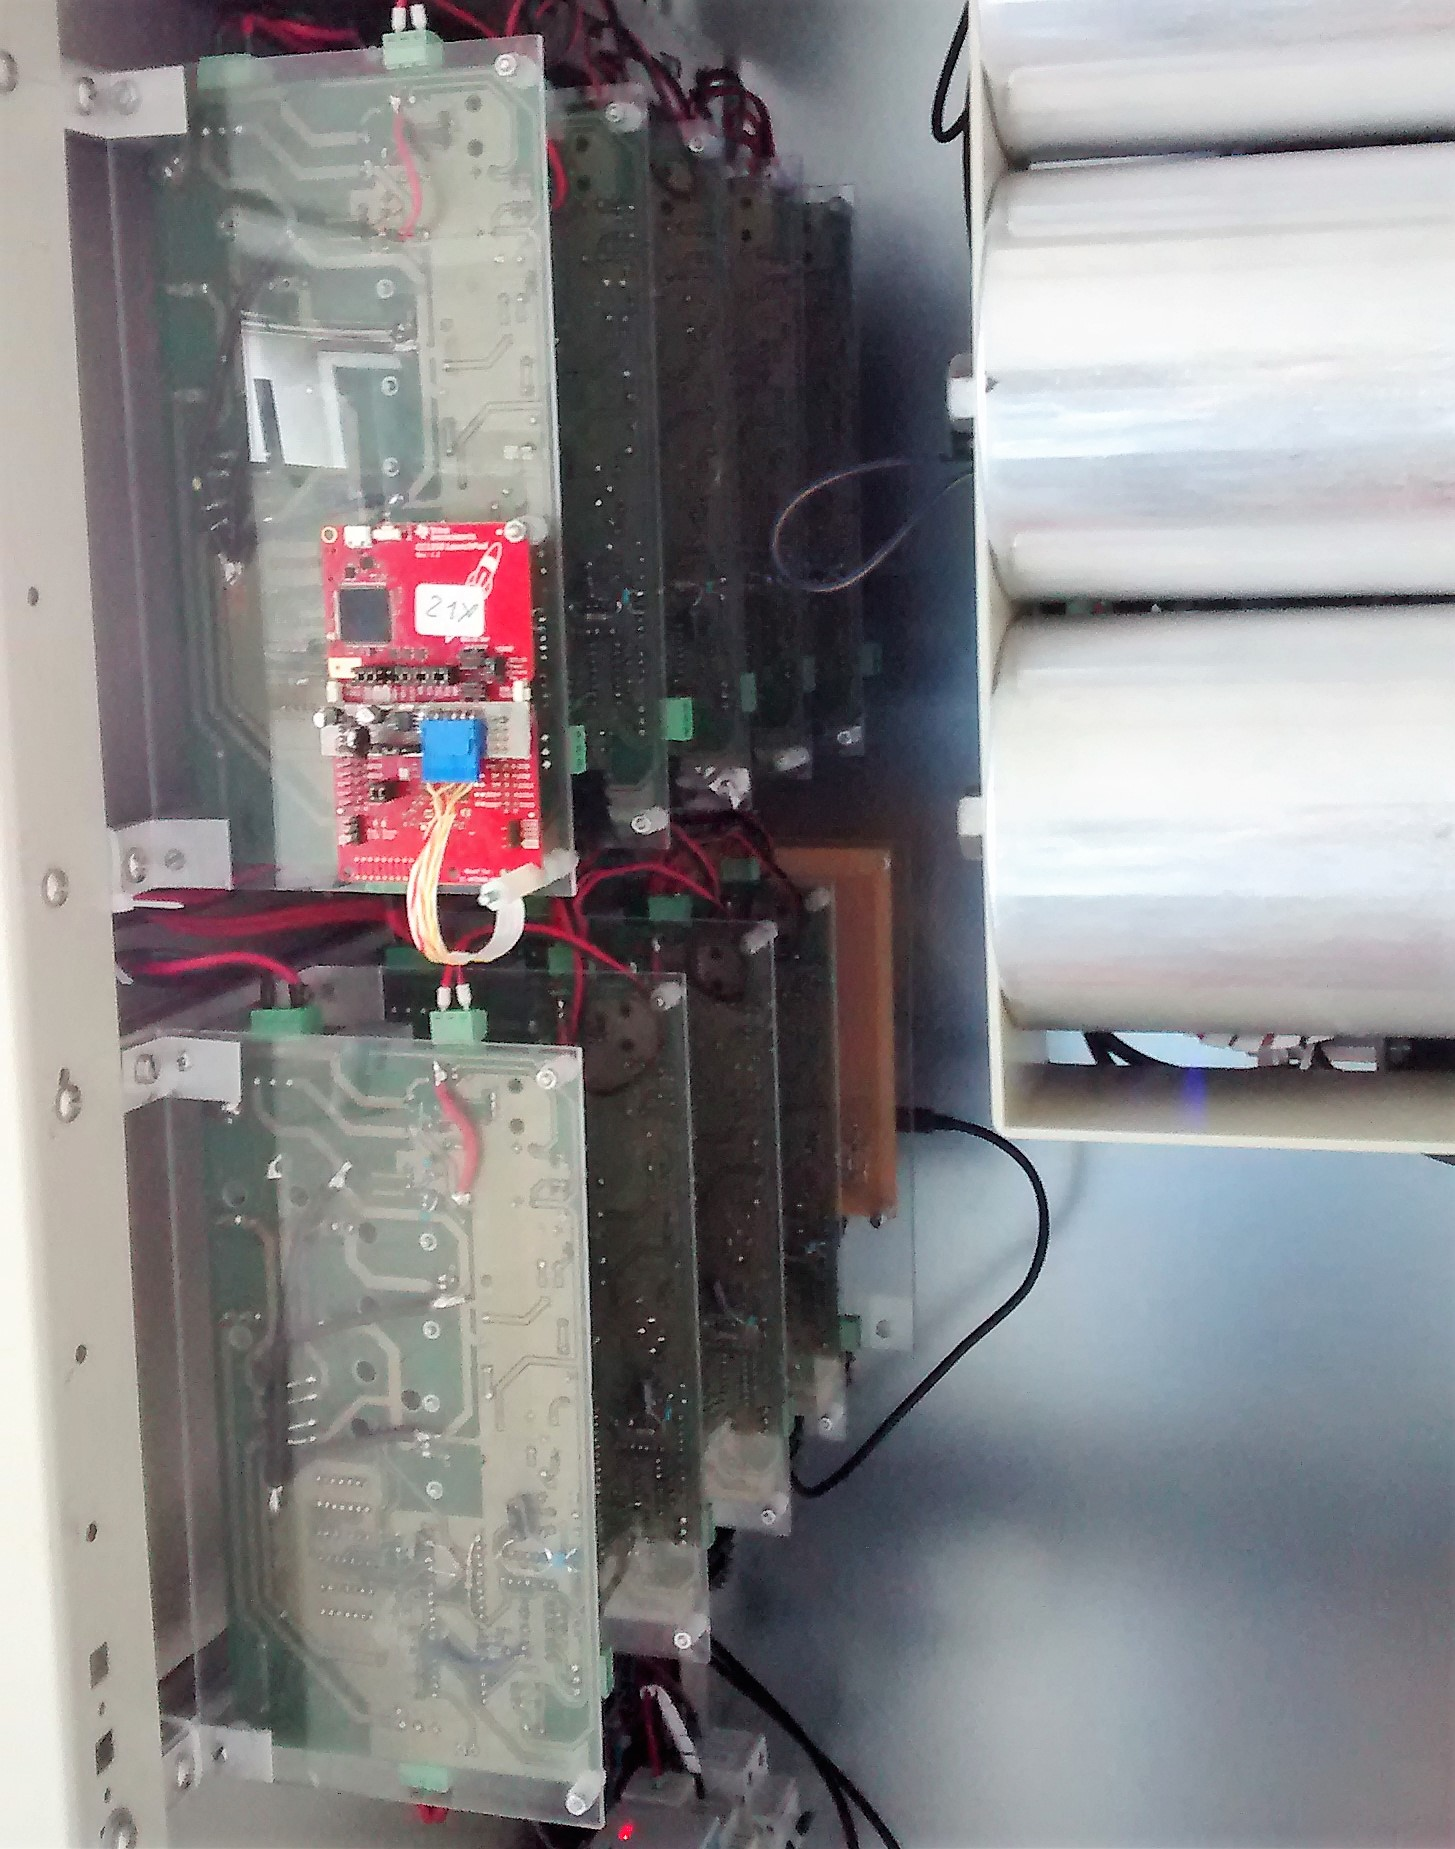
\includegraphics[width=0.98\linewidth, keepaspectratio]{figures/armario2}
		\caption{Detail of wireless module}
		\label{fig:3.4.armario2}
	\end{minipage}
\end{figure}

\subsection{Validating the electric measurements}

The first results collected by the wireless node are presented in figure \ref{fig:3.4.measurements}.
Identified in red in the graph are presented the three electric tests: a) increase of the DC\_bus voltage with a voltage controlled source; b)increase of the DC current in the PV current transducer, with a current controlled source; c) Increase of the PV DC voltage, with a voltage controlled source. As a consequence of the power converter topology, the DC\_bus voltage increases due to a diode between two sides of the converter.



\begin{figure}[h!]
	\centering
	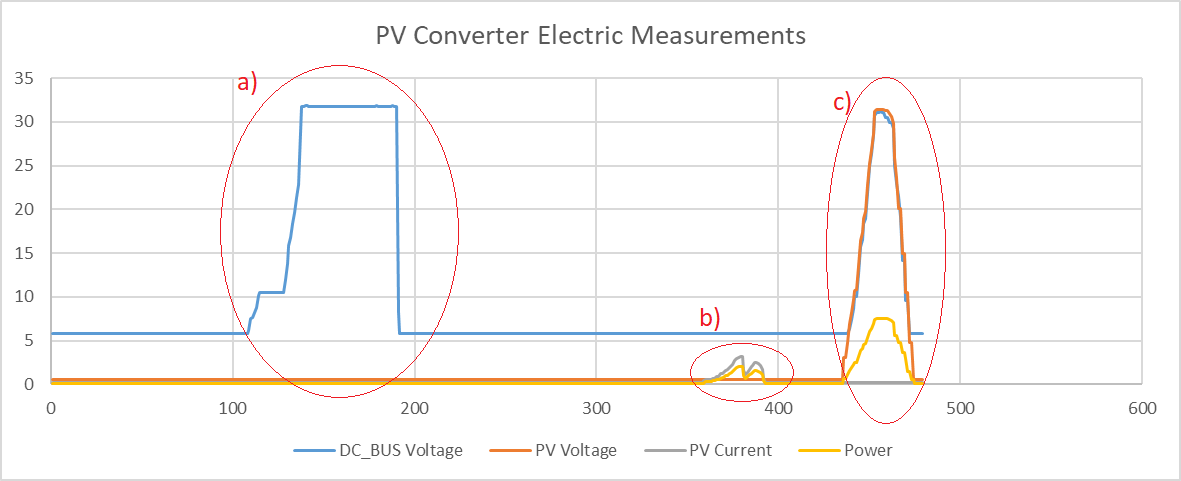
\includegraphics[width=0.85\textwidth,keepaspectratio]{figures/measurements}
	\caption{PV power converter electric measurements. (horizontal axis in seconds)}
	\label{fig:3.4.measurements}
\end{figure}

\subsection{Validating the wireless communication}
The Texas Instruments WSN implementation used evaluates the wireless strength of the received data. In figure \ref{fig:3.4.rssi} is presented the Received Signal Strength Indication (RSSI), as a measurement of the power present in a received radio signal. 


\begin{figure}[h!]
	\centering
	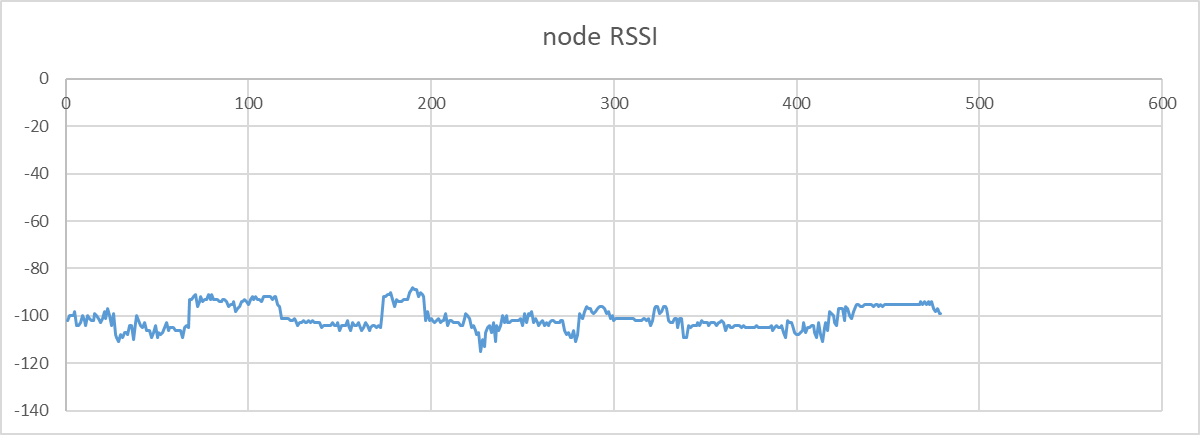
\includegraphics[width=0.85\textwidth,keepaspectratio]{figures/RSSI}
	\caption{PV power converter electric measurements. (horizontal axis in seconds)}
	\label{fig:3.4.rssi}
\end{figure}

Complementary, the existence of multiple nodes was validated, as presented in the raw data of the concentrator verified in figure \ref{fig:3.4.twonodes}.


\begin{figure}[h!]
	\centering
	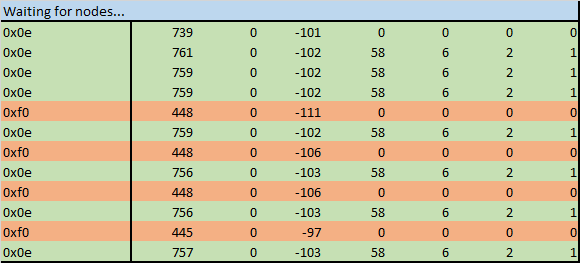
\includegraphics[width=0.80\textwidth,keepaspectratio]{figures/twonodes}
	\caption{Concentrator raw data received.}
	\label{fig:3.4.twonodes}
\end{figure} 


%\section{Discussion of the results}
%\label{sec:3.5}
%\lipsum[4-4]

